\chapter{The framework}
\label{chap:framework}

This chapter presents the design and implementation of the framewor which was developed as part of this thesis.
It list the requirements of the framework, goes through its development lifecycle and presents the architecture of the framework.

This framework, which is the main contribution of this thesis, allows for a fair comparison of the considered algorithms by having them implemented in a common environment
and language, in order to avoid performacne differences induced by the programming language, and by having them run on the exact same benchmark problem implementations and
settings.

The code for the framework is available at \url{https://github.com/MSc-Thesis-Samy/code} and includes a README file with instructions on how to use it.

\section{Requirements}

\subsection{Goals and functional requirements}

The overreaching goal of the framework is to provide a tool for the evaluation of neuroevolution algorithms on benchmark problems, based on the selection
presented in \Cref{chap:review}.
Tests are specified through a command line interface, they consist in an algorithm and problem pair, along with a set of additional parameters.
The framework collects the results of the tests as well as the list of passed-in parameters, algorithm and problem.
These tests can either be run individually or in batch mode, where the framework runs a set of tests in parallel, and collects statistics on these runs.

Furthermore, the framework also allows for the visualization of the problem, solution process and network structure through a graphical user interface.

\subsection{Non-functional requirements}

Non-functional requirements are the requirements that specify the quality of the system, rather than the features it should have.
Apart from the functional requirements that specify the features expected of the framework, a number of non-functional requirements have also been identified.

\begin{itemize}
    \item Usability and user experience: the framework should be easy to use and provide a good user experience.
    \item Documentation: The framework should be well documented, providing a clear and concise guide on how to use it.
    \item Error handling: All errors should be handled gracefully as to not result in runtime errors.
    \item Performance: The framework should allow for the execution of tests in parallel, making use of multiple CPU cores.
    \item:Extensibility: The framework should be easily extensible, allowing for the addition of algorithms and benchmarks without any
    major changes to the existing codebase.
    \item Support: The framework should be able to run on the three major operating systems: Windows, Linux and MacOS.
\end{itemize}

\section{Architecture}

The framework is implemented in Rust. This general-purpose programming language, originally intended to serve as an alternative for system languages such as C and
C++, offers a good balance between performance provided by such low-level languages and the safety and ease of use of higher-level languages such as Python.
Furthermore, various libraries (referred to as Rust crates) which could be used when implementing aspects of the framework, such as designing the command-line interfaces
and graphical-user interfaces, or running CMA\_ES are available in Rust.
Lastly, the language can target a range of platforms, including Windows, Linux and MacOS.

The framework is divided into three main components:

\begin{itemize}
    \item The core: This component is responsible for the execution of the tests and the collection of results. It contains the algorithms and benchmark implementations.
    \item The command-line interface: This component allows the user to specify the tests to be run, as well as the parameters for these tests.
    \item The graphical user interface: This component allows the user to visualize the problem, solution process and network structure, as well as the test results.
\end{itemize}

The core is used by both the command line interface and the graphical user interface. And the graphical user interface is used by the command line interface.
Indeed, the UI allows for the visualization of the solution process, but interaction with the framework is done when invoking it through the command line interface.

The dependency graph of the framework is shown in \Cref{fig:dependency_graph}.

\begin{figure}
    \centering
    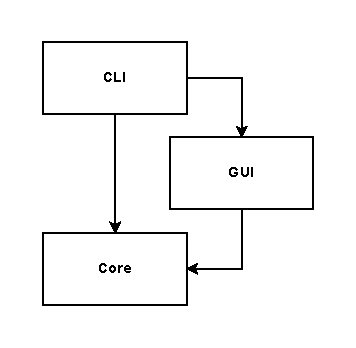
\includegraphics[width=0.5\textwidth]{Pictures/dependency}
    \caption{Dependency graph of the framework}
    \label{fig:dependency_graph}
\end{figure}

\subsection{Background on Rust features}

This section provides a brief overview of the features of the Rust programming language before going into the details of the framework's implementation.

\subsubsection{Object-oriented capabilities}

Nowadays, object-oriented languages are considered the norm for the development of large-scale software systems in the industry.
Rust is inspired by various programming paradigms, such as functional programming and object-oriented programming.
Although there is no consensus on the list of features which define an object-oriented programming language, Rust can be considered object-oriented.
Indeed, it allows for the definition of structs and enums which can store data and methods using implementation blocks.

It also allows for encapsulation through the use of the \texttt{pub} keyword, which specifies the visibility of objects, thus defining the public API for interacting
with them. When not using the \texttt{pub} keyword, the object is private and can only be accessed by the module it is defined in.
Modules are used to organize code and define the visibility of objects, and can be nested to form a hierarchy.
However, a major difference with other object-oriented languages such as Java or C\# is that Rust does not have a class-based inheritance system.
Instead, it takes a different approach which consists in polymorphism, which is a more general system referring to code that can work with multiple types.
In practice, this is achieved through the use of generics in method and object definitions, and the use of traits, which are similar to interfaces in other languages.
In fact, traits allow for the definition of a default implementation for a set of methods, which can be overridden by the implementing type.

\subsubsection{Enums}

Enums are a powerful feature of Rust, which allow for the definition of a type through the enumeration of its possible variants.
They are used in combination with pattern matching, which allows for the deconstruction of an enum and the extraction of its values.
Together, these two features allow for the definition of complex types and the implementation of algorithms in a concise and readable way, and are widely used in the
framework.

\subsubsection{Library management}

Cargo is Rust's build system and package manager. Most projects are managed using this tool which handles the download and building of the dependencies of projects.
In Rust, packages are referred to as crates.

\subsubsection{Attributes}

Attributes are metadata applied to some module, crate or object. They are, for example, used to enable compiler features or mark functions as unit tests.
or to define the behavior of the code. They are defined using the \texttt{\#} symbol and are placed before the object they are associated with.

\subsubsection{Testing}

In Rust, unit-testing is usually done by defining a test module (with a test attribute) at the end of the file containing the functionalities to be
tested. Test functions correspond to functions defined in such modules, which are marked with a specific test attribute. They can be run
with \texttt{cargo test} and fail when a \textit{panics} occur.  Utility macros such as \texttt{asserteq} or \texttt{assert} can be used to panic
when conditions are not met.

\subsubsection{Concurrency}

Concurent programming refers to different parts of a program executing independently of each other, while parallel programming refers to different parts
of a program executing in parallel, at the same time. For simplicity, in this section, "concurrency" should be understood as "concurrency and/or parallelism".
These concepts have become particularly important in the context of modern computing, where multi-core processors are the norm. However, writing concurrent
programs can be difficult, as it can be error-prone, hard to debug and reason about. Rust aims at addressing these issues by making it use of its main feature:
the borrowing and ownership system, which allows many concurrency issues to be caught at compile time, rather than at runtime, as it is the case in other languages.
In Rust, concurrency is achieved through the use of threads, which are lightweight processes that can run concurrently. The standard library provides
various methods for creating and managing threads. However, in this project, the \texttt{rayon} crate is used instead. It is a data parallelism library
which allows for a particularly easy way to parallelize code, by providing parallel iterators and parallel maps, and abstracting away the details of
thread creation and management, guaranteeing data-race free execution and benefiting from parallelism when possible.

For example, \Cref{lst:sum_of_squares} shows how a function \texttt{sum\_of\_squares}, which computes the sum of the squares of the elements of an array.
By simply using the \texttt{par\_iter} method from the \texttt{rayon} crate, instead of the \texttt{iter} method, the function can be parallelized, as demonstrated
by the \texttt{sum\_of\_squares\_parallel} function.

\begin{lstlisting}[label=lst:sum_of_squares,caption=Sum of squares,float,frame=tb]
use rayon::prelude::*;

fn sum_of_squares(input: &[i32]) -> i32 {
    input.iter().map(|x| x * x).sum()
}

fn sum_of_squares_parallel(input: &[i32]) -> i32 {
    input.par_iter().map(|x| x * x).sum()
}
\end{lstlisting}


\subsection{Core}

This component contains the core functionality of the framework

Various constants and utility functions, used across the project, are defined in the \texttt{utils.rs} and \texttt{constants.rs} files.

\subsubsection{Algorithms}

The algorithms are implemented as structs and are accessed as variants of an \texttt{Algorithm} enum, which lists all the implemented algorithms.
The algorithm structs and the \texttt{Algorithm} enum implement the \texttt{NeuroevolutionAlgorithm} trait, which defines the methods that an algorithm must implement.
These methods are:

\begin{itemize}
    \item \texttt{evaluate}: This method takes as input a vector of floats and returns the output of the algorithm on this input.
    \item \texttt{optimization\_step}: This method takes as input a problem and performs an optimization step on the algorithm.
    \item \texttt{optimize}: This method takes as input a problem and a number of iterations, and performs successive optimization steps on the algorithm.
        It is implemented as a default method, which calls the \texttt{optimization\_step} method in a loop.
    \item \texttt{optimize\_with\_early\_stopping}: This method takes as input a problem, a number of maximum iterations, a tolerance value and an optional number of
        stagnation iterations. It performs optimization steps on the algorithm, stopping when the maximum number of iterations is reached, when the fitness value
        is close enough to the optimal value (based on the passed-in tolerance) or when the fitness value has not improved for a number of iterations (based on the
        passed-in stagnation iterations). It is also implemented as a default method at the trait level.
\end{itemize}

The \texttt{Algorithm} enum and the \texttt{NeuroevolutionAlgorithm} trait are defined in the \\ \texttt{neuroevolution\_algorithm.rs} file.
Each of the different algorithm structs are defined in their own file, such as \texttt{neat.rs} or \texttt{vnetwork.rs}.

For the CMA-ES algorithm, the \texttt{cmaes} crate \footnote{\url{https://docs.rs/cmaes/latest/cmaes/}}  is used. An external library was used instead of implementing
the algorithm from scratch in the framework because of the popularity of CMA-ES, which led to the devlopment of high quality and trusted libraries for different programming
languages, and because the focus of the thesis regarding this algorithm is not on the CMA-ES algorithm itself, as its default parameters can already be applied to problems, but
on the topology of the used networks.

As described in \Cref{chap:review}, the computation of outputs for these two algorithms consist in checking whether or
not the input is above hyperplanes in the case of (1 + 1) NA, or in cones in the case of BNA. The following two paragraphs described how this is done in the framework.

\paragraph{Computation for (1 + 1) NA in practice: }
The ANNs which are evolved using the (1 + 1) NA algorithm output the union of $N$-dimensional hyperplanes. To check whether or not the input is above the
hyperplane described by one of the neurons, the normal vector $\overrightarrow{n}$ to the hyperplane is computed using the angles and a norm of $1$.
For an input vector $\overrightarrow{x}$, the dot product $(\overrightarrow{x} - \lvert b \rvert \overrightarrow{n}) \cdot \overrightarrow{n}$ is computed, where
$b$ is the bias of the neuron. If $b \geq 0$, the output of the neuron is $1$ if the dot product is positive and $0$ otherwise. If $b < 0$,
the output of the neuron is $1$ if the dot product is negative and $0$ otherwise.

\paragraph{Computation for BNA in practice: }
V-neurons output whether or not the input is in the cone described by the neuron. The vector $\overrightarrow{\varphi}$ is computed using the angles $\varphi_1, \ldots, \varphi_{D-1}$
and a norm of $1$. Given an input vector $\overrightarrow{x}$, the dot product $(\overrightarrow{x} - \lvert b \rvert \overrightarrow{\varphi}) \cdot \overrightarrow{\varphi}$ is computed.
The angle $\alpha$ between the input vector and the normal vector can then be computed as
$\alpha = \cos^{-1}(\frac{(\overrightarrow{x} - \lvert b \rvert \overrightarrow{\varphi}) \cdot \overrightarrow{\varphi})}{\lVert \overrightarrow{x} - \lvert b \rvert \overrightarrow{\varphi} \rVert
\lVert \overrightarrow{\varphi} \rVert})$. If $b \geq 0$, the output of the neuron is $1$ if $\alpha \leq \theta$ and $0$ otherwise. If $b < 0$, the output of the neuron is
$1$ if $\pi - \alpha \leq \theta$ and $0$ otherwise.

\subsubsection{Benchmarks}

The problems are implemented as variants of a \texttt{Benchmark} enum, and are defined in the \texttt{becnhmarks.rs} file.
This enum contains four variant, for each of the implemented benchmark types: \texttt{PoleBalancing}, \texttt{Classification}, \texttt{SphereClassification}
and \\ \texttt{DatasetClassification}.
The classification variants hold an instance of the \texttt{LabeledPoints} type, storing the labeled data.
Because of the presence of a training and testing set in the case of the \texttt{DatasetClassification} variant, the variant stores two instance of this type.
The file contains functions to generate the
data for each of the classification problems, i.e, parsing it from a text file for the \textit{Cancer1} problem, or iterating other
angle values for the sphere classification problems. In particular, the \texttt{Benchmark} enum defines a \texttt{evaluate} method, taking as input an
algorithm (an instance of the \texttt{Algorithm} enum) and which returns the fitness of the algorithm on the task.
It also defines a \texttt{test} method, which generally behaves the same as the \texttt{evaluate} method, except for dataset classification problems, where
the fitness is computed on the testing set, as opposed to the training set in the \texttt{evaluate} method.

\paragraph{Classification problems} For the sphere classification and dataset classification tasks, the fitness is computed using the \texttt{classification}
function from the \texttt{benchmarks.rs} file, which computes the $MAE$ (Mean Absolute Error) \footnote{\url{https://en.wikipedia.org/wiki/Mean_absolute_error}}
For the bna and (1 + 1) NA algorithm, which output boolean
values, this is equivalent to computing the accuracy (i.e, the number of correct predictions divided by the number of total predictions), while also
allowing for the evaluation of the CMA-ES and NEAT method, outputting probables when using the sigmoid activation on the output neuron.

\paragraph{Pole Balancing} The logic for the pole balancing simulation is implemented in the  \\ \texttt{pole\_balancing.rs} file, where the state is defined, along with methods
responsible for updating it based on the dynamic equations and the Euler method. The \texttt{pole\_balancing} function in the \texttt{benchmarks.rs} file simply
updates the state, using the scaled algorithm output as the applied force, and checking whether or not the success conditions for the task are still met.

\subsubsection{Testing}

Unit-tests were implemented across the core component to test the behavior of the algorithms and benchmarks.
These tests were implemented in parallel with the functionalities to avoid and identify potential bugs early in the development process before
building up with more functionalities. In addition, they were ran at each new push to github using a workflow responsible for compiling the project,
targeting linux, and running all the tests. This is to ensure that new changes do not break any past working functionality.

In fact, the bna and $(1 + 1)$ NA problems were tested using the sphere classification problems, where optimal solutions are known. These tests
consist in checking whether one of these algorithms, with parameters corresponding to an optimal solution, does indeed lead to a maximum fitness value
of $1.0$. These tests are defined in the \texttt{benchmarks.rs} file. For example, the \texttt{test\_half\_network} function checks that a decision line
corresponding to the x-axis for the continuous $(1 + 1)$ NA algorithm gives a fitness of $1.0$. For the BNA algorithm, where there are infinitely many
solutions to the sphere classification problems, different solutions were checked.

Furthermore, two additional tests in the \texttt{benchmarks.rs} file are responsible for checking that the data is loaded properly from the \textit{cancer}
text file. Tests in the \texttt{pole\_balancing.rs} file test the physics of the simulation implementation, for example verifying that a pole at the lowest
position, with no external force, does not lead to any movement of the cart or the pole.

Lastly, regarding the CMA-ES and NEAT algorithms, the behavior of their core functions was tested. Test functions in the \texttt{neat.rs} test the
behavior of functions such as the crossover or initialization, using examples from the original paper \cite{neat} when available. The functions in
\texttt{neural\_network.rs} test the output of the feed-forward method and activation functions.

\subsection{Command-line interface}

The command lien interface is implemented using the \texttt{clap} crate, which is a widely used command line argument parser in Rust.
It allows for the execution of tests, by providing the algorithm, the problem and additional parameters. These additional parameters are optional and have
default values, they are used to specify parameters for the algorithms, such as the number of neurons, parameters for the optimization, such as the number of
iterations, and toggling the visualization of the solution process and network structure.

Arguments can be of three different types:

\begin{itemize}
    \item \textbf{Positional}: These are required arguments which are specified in the order they are defined in the command line interface.
    \item \textbf{Named}: These are optional arguments which are specified by their name and a value.
    \item \textbf{Flags}: These are optional arguments which are specified by their name and are either present or not.
\end{itemize}

The \texttt{Cli} struct is defined in the \texttt{cli.rs} file, it contains members for each of the command line arguments and derives the \texttt{Parser} trait.
The argument name is set to the member name, a short name,help message, default value and the argument type are specifies in an attribute on the member.

The arguments are parsed in the \texttt{bin/main.rs} file, which is the entry point of the program.

In order to ensure that the passed-in arguments are valid, the rust type system is leveraged, specifying appropriate data types for each of the argument.
For example, the iteration number is set to an unsigned integer \texttt{u32}, while the algoithm and benchmarks are set to two enums, \texttt{AlgorithmType} and
\texttt{Problem}, with variants for each possible option.

The command line interface is shown in \Cref{verb:cli}. Parameters for the BNA and $(1 + 1)$ NA algorithms are passed in as named arguments. For NEAT and CMA-ES, where more
parameters can be specified, the path to \texttt{.toml} configuration files are passed-in instead. Examples of such configuration files are shown in \ref{verb:cmaes_config}
and \ref{verb:neat_config}. The CMA-ES configuration file is used to specify the fixed network topology and activation functions, while the NEAT configuration file
is used to specify the various parameters of the algorithm. Some configuration files are provided in the \texttt{config} directory and more examples can be found in
\Cref{app:configurations}.

\begin{lstlisting}[label=verb:cmaes_config,caption=Example of a configuration file for CMAE-ES,float,frame=tb]
input_ids = [1, 2]
output_ids = [5]
bias_id = 3

[[neurons]]
id = 4
inputs = [1, 2, 3]
activation = "sigmoid"

[[neurons]]
id = 5
inputs = [1, 2, 3, 4]
activation = "sigmoid"
\end{lstlisting}

\begin{lstlisting}[label=verb:neat_config,caption=Example of a configuration file for NEAT,float,frame=tb]
population_size = 150
n_inputs = 2
n_outputs = 1
weights_mean = 0.0
weights_stddev = 0.8
perturbation_stddev = 0.2
new_weight_probability = 0.1
enable_probability = 0.25
survival_threshold = 0.25
connection_mutation_rate = 0.3
node_mutation_rate = 0.03
weight_mutation_rate = 0.8
similarity_threshold = 15.0
excess_weight = 1.0
disjoint_weight = 1.0
matching_weight = 0.3
champion_copy_threshold = 5
stagnation_threshold = 1500
\end{lstlisting}

\begin{lstlisting}[label=verb:cli,caption=Command line interface,float,frame=tb]
Neuroevolution framework for testing algorithms on benchmark problems.

Usage: main [OPTIONS] <ALGORITHM> <PROBLEM>

Arguments:
  <ALGORITHM>  The algorithm to test [possible values: oneplusonena, bna, neat, cmaes]
  <PROBLEM>    the benchmark problem [possible values: half, quarter, two-quarters, square, cube, xor, pole-balancing, proben1, local-opt]

Options:
  -r, --resolution <RESOLUTION>  Resolution, when applicable [default: 1000]
  -i, --iterations <ITERATIONS>  Number of iterations [default: 500]
  -n, --neurons <NEURONS>        Number of neurons, when applicable [default: 1]
  -g, --gui                      Display visualization
  -f, --file <FILE>              Configuration file
  -o, --output <OUTPUT>          Results output file
  -t, --test-runs <TEST_RUNS>    Number of runs
  -e, --error-tol <ERROR_TOL>    Max fitness tolerance [default: 0.02]
  -s, --stagnation <STAGNATION>  Max stagnation
  -h, --help                     Print help
  -V, --version                  Print version
\end{lstlisting}

\subsection{Graphical user interface}

The UI is implemented using the \texttt{ggez} \footnote{\url{https://ggez.rs}} crate, which is intended to be a simple 2D game framework.
In particular, it provides a simple interface for creating windows, drawing geometrical shapes and handling user input.
This crate relies on the definition of a \texttt{State} struct, which holds the parameters of the game state, and which implements the \texttt{EventHandler} trait.
This trait defines two methods: \texttt{update}, which is used for updating the state, and \texttt{draw} which is used for rendering the state.
These two methods are called by the game loop, which is triggered in the \texttt{bin/main.rs} file if the \texttt{gui} flag is set when invoking the program.

This game abstraction is particularly suited for the implementation of visualization in the framework.
The \texttt{State} struct defined in \texttt{gui.rs} holds an \texttt{algorithm}, a \texttt{problem}, and two additioal members keeping track of the number of iterations.
An instance of this struct is created in the \texttt{bin/main.rs} file using the arguments passed in the command line interface.
The \texttt{update} method updates the \texttt{algorithm} by running an optimization step, and the \texttt{draw} renders the different visualizations, based on
the \texttt{problem} and \texttt{algorithm} members.

The number of iterations and the best fitness value are shown in the top left corner of the window.

\subsubsection{Classification problems}

For the sphere classification problem, the unit-sphere is shown, along with its points which are labeled as \texttt{true}, which are shown in green, and its points
labeled as \texttt{false} which are shown in red. When running the (1 + 1) NA algorithm, the decision line and normal vector are shown. In the case of the BNA algorithm,
the normal vector and decision cones are shown. For the CMA-ES and NEAT algorithms, the output of the network is shown, as a gradient of colors, with the green
corresponding to the highest values and the red to the lowest values.
Similarly, for the \textit{XOR} problem, the only difference is that the unit-sphere is not shown.
No visualization is shown for the higher dimension \textit{Proben1 Cancer1} problem.

\subsubsection{Pole balancing}

The visualization of the pole balancing problem consists in drawing the cart and pole, and updating their position based on the state of the simulation.
It is implemented in the \texttt{pole\_balancing\_gui.rs} file. Compared to the classification problems, where the visualization is updated as the algorithm is evolved in the \texttt{update} method,
the pole balancing visualization does not update the passed-in algorithm, but rather updates the simulation state based on the output of the algorithm.

Screenshots of the GUI for different problems and algorithms are shown in \Cref{fig:gui_screenshots}.

\begin{figure}
    \centering
    \begin{subfigure}{0.5\textwidth}
        \centering
        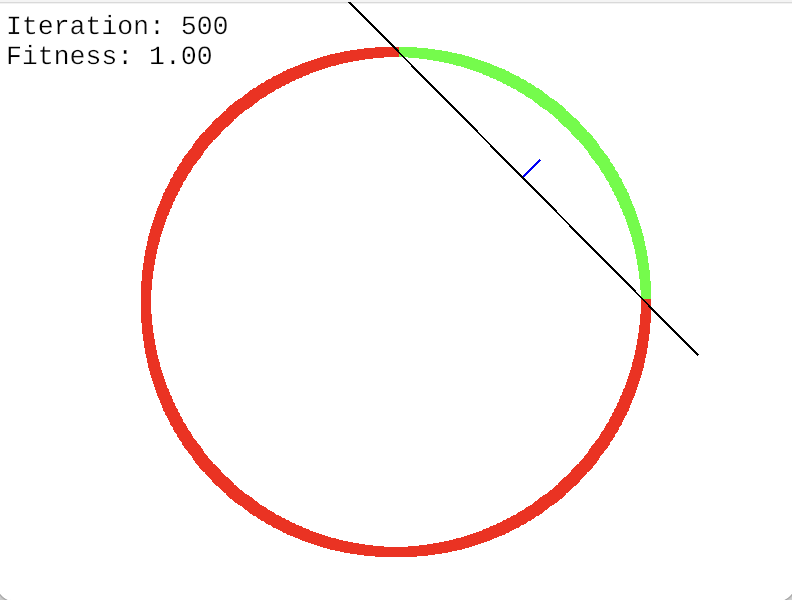
\includegraphics[width=0.8\linewidth]{Pictures/oneplusonena_gui}
        \caption{(1 + 1) NA on \textit{Quarter}}
    \end{subfigure}%
    \hfill
    \begin{subfigure}{0.5\textwidth}
        \centering
        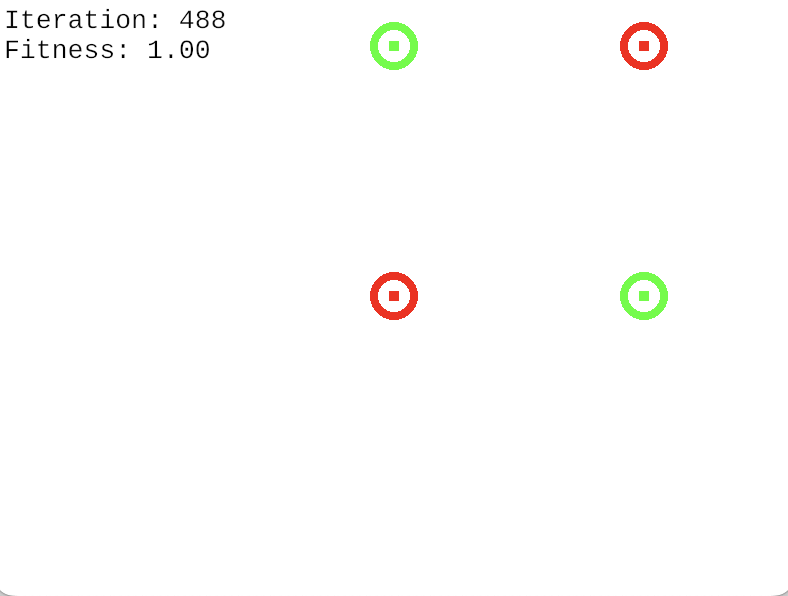
\includegraphics[width=0.8\linewidth]{Pictures/xor_gui}
        \caption{NEAT on \textit{XOR}}
    \end{subfigure}%
    \hfill
    \begin{subfigure}{0.5\textwidth}
        \centering
        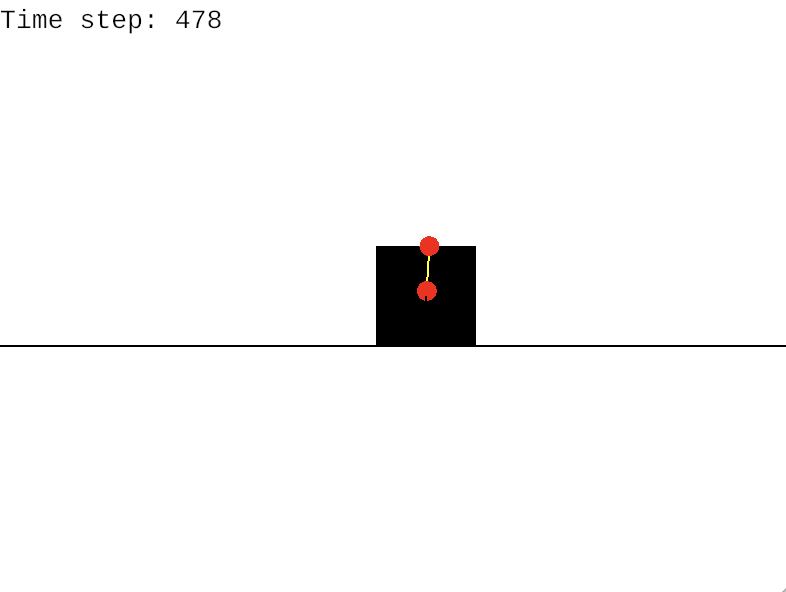
\includegraphics[width=0.8\linewidth]{Pictures/pole_balancing_gui}
        \caption{Pole balancing simulation}
    \end{subfigure}%
    \hfill
    \begin{subfigure}{0.5\textwidth}
        \centering
        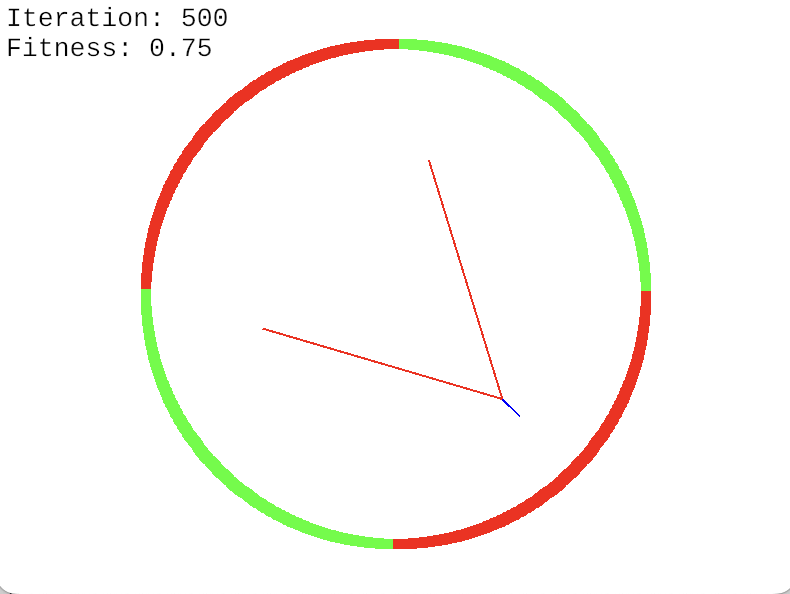
\includegraphics[width=0.8\linewidth]{Pictures/bna_gui}
        \caption{BNA on \textit{TwoQuarters}}
    \end{subfigure}%
    \hfill
    \begin{subfigure}{0.5\textwidth}
        \centering
        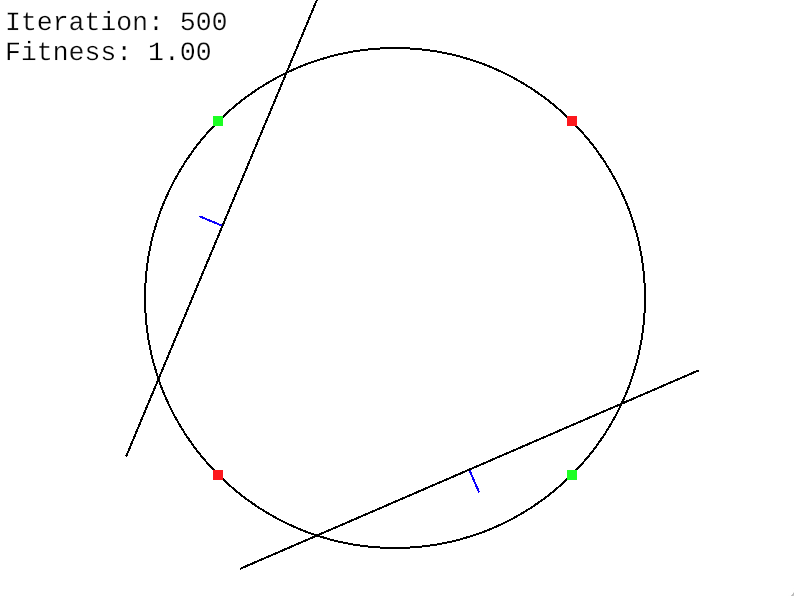
\includegraphics[width=0.8\linewidth]{Pictures/oneplusonena_xor_gui}
        \caption{(1 + 1) NA on \textit{XOR}}
    \end{subfigure}%
    \hfill
    \begin{subfigure}{0.5\textwidth}
        \centering
        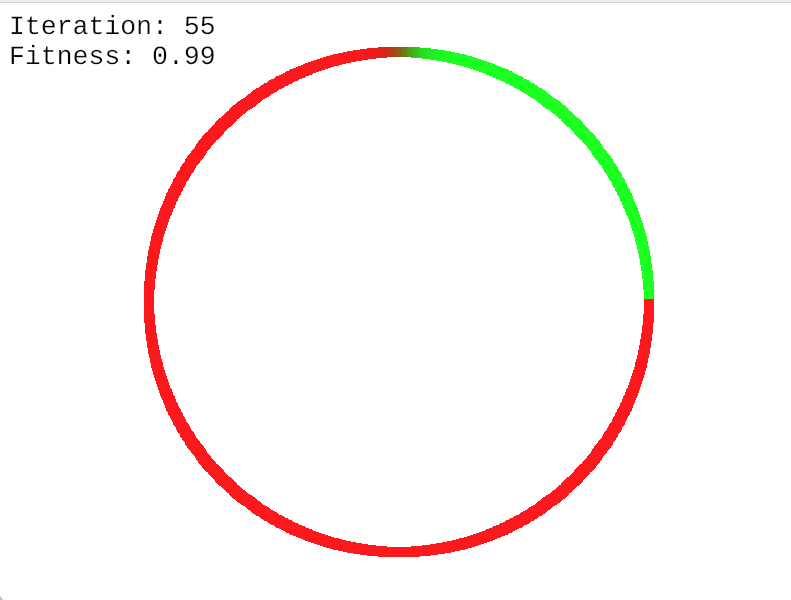
\includegraphics[width=0.8\linewidth]{Pictures/neat_sphere_gui}
        \caption{NEAT on \textit{Quarter}}
    \end{subfigure}%
    \caption{Examples of the GUI visualizations for different problems and algorithms}
    \label{fig:gui_screenshots}
\end{figure}
